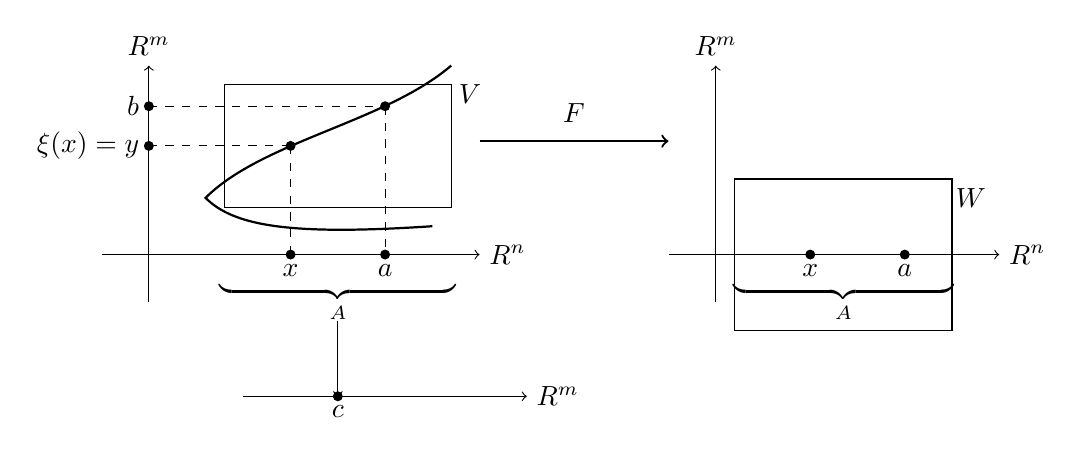
\begin{tikzpicture}[scale=1.2]

  % Ejes izquierda
  \draw[->] (-3,-0.5) -- (-3,2) node[above] {$\mathbb{R}^m$};
  \draw[->] (-3.5,0) -- (0.5,0) node[right] {$\mathbb{R}^n$};

  % Conjunto A (intervalo)
  \draw (-2,0) -- (0,0);
  \node at (-1,-0.5) {
    $\underbrace{\hspace{3cm}}_{A}$
  };

  % Puntos en A
  \fill (-1.5,0) circle (1.5pt) node[below] {$x$};
  \fill (-0.5,0) circle (1.5pt) node[below] {$a$};
  \fill (-0.5,1.57) circle (1.5pt);
  \fill (-1.5,1.15) circle (1.5pt);
  \fill (-3,1.57) circle (1.5pt) node[left] {$b$};
  \fill (-3,1.15) circle (1.5pt) node[left] {$\xi(x)=y$};
  \draw[dashed] (-3,1.57) -- (-0.5,1.57);
  \draw[dashed] (-0.5,1.57) -- (-0.5,0);
  \draw[dashed] (-3,1.15) -- (-1.5,1.15);
  \draw[dashed] (-1.5,1.15) -- (-1.5,0);
  
  % Rectángulo (V)
  \draw (-2.2,0.5) rectangle (0.2,1.8);
  \node at (0.4,1.7) {$V$};
  
  % Curva dentro
      \draw[thick] 
      (0,0.3) 
      .. controls (-1.5,0.2) and (-2.1,0.3) .. (-2.4,0.6)
      .. controls (-1.8,1.2) and (-0.5,1.4) .. (0.2,2);
  
  % Flecha F
  \draw[->, thick] (0.5,1.2) to[out=0,in=180] (2.5,1.2);
  \node at (1.5,1.5) {$F$};
  
  % Ejes derecha
  \draw[->] (3,-0.5) -- (3,2) node[above] {$\mathbb{R}^m$};
  \draw[->] (2.5,0) -- (6,0) node[right] {$\mathbb{R}^n$};
  
  
  % Rectángulo (W)
  \draw (3.2,-0.8) rectangle (5.5,0.8);
  \node at (5.7,0.6) {$W$};
  
  % Conjunto A (intervalo)
  \draw (-2,0) -- (0,0);
  \node at (4.35,-0.5) {
      $\underbrace{\hspace{2.8cm}}_{A}$
  };
  
  % Puntos imagen
  \fill (4,0) circle (1.5pt) node[below] {$x$};
  \fill (5,0) circle (1.5pt) node[below] {$a$};
  
  % Flecha hacia abajo (A a c)
  \draw[->] (-1,-0.7) -- (-1,-1.5);
  
  % Línea inferior
  \draw (-2,-1.5) -- (0,-1.5);
  \fill (-1,-1.5) circle (1.5pt) node[below] {$c$};
  \draw[->] (0,-1.5) -- (1,-1.5) node[right] {$\mathbb{R}^m$};

\end{tikzpicture}
